\documentclass{beamer}
\usepackage[T1]{fontenc}
\usepackage[utf8]{inputenc}
\usepackage[cyr]{aeguill}
\usepackage[english]{babel}
\usepackage{amsmath,amssymb,amsthm}
\usepackage{bm}
\usepackage{graphicx}
\usepackage{geometry}
\usepackage{tikz}
\usepackage{diffcoeff}
\usepackage{tcolorbox}

 %%BeginIpePreamble
\usepackage{amsfonts}
%%EndIpePreamble

\usepackage{comment}

\usepackage[backend=bibtex]{biblatex}
\makeatletter
\def\blx@maxline{77}
\makeatother

\bibliography{biblio_presCPDE}
\AtBeginBibliography{\small}

\usepackage{multirow}
\usepackage[justification=centering]{caption}
\usepackage{subfig}
\usepackage{xcolor,colortbl}

\newcommand{\mc}[2]{\multicolumn{#1}{c}{#2}}
% normal box
\newcommand{\sqboxs}{1.2ex}% the square size
\newcommand{\sqboxf}{0.6pt}% the border in \sqboxEmpty
\newcommand{\sqbox}[1]{\textcolor{#1}{\rule{\sqboxs}{\sqboxs}}}

\definecolor{Blue}{rgb}{0,1,1}
\definecolor{Green}{rgb}{0.4,1,0.4}
\definecolor{GreenYellow}{rgb}{0.3,0.6,0.5}
\definecolor{Yellow}{rgb}{1,1,0.4}
\definecolor{Orange}{rgb}{1,0.6,0.2}
\definecolor{Purple}{rgb}{1,0.5,0.5}
\definecolor{Red}{rgb}{1,0.2,0.2}

\definecolor{Grey}{rgb}{0.5,0.5,0.5}

\newcolumntype{g}{>{\columncolor{Green}[1\tabcolsep]}c}
\newcolumntype{m}{>{\columncolor{Yellow}[1\tabcolsep]}c}
\newcolumntype{b}{>{\columncolor{Blue}[1\tabcolsep]}c}
\newcolumntype{N}{>{\setbox0=\hbox\bgroup}c<{\egroup}@{}}

\usepackage{multimedia}

\graphicspath{{./Figures/},{./Videos/}}

\newtheorem{remark}{Remark}
\newtheorem{proposition}{Proposition}

\makeatletter \renewcommand\d[1]{\ensuremath{%
		\;\mathrm{d}#1\@ifnextchar\d{\!}{}}}
\makeatother

\mode<presentation> {
	%\usetheme{Singapore}
	\usetheme{Madrid}
}
\usefonttheme{serif}

\DeclareMathOperator*{\argmax}{arg\,max}
\DeclareMathOperator*{\argmin}{arg\,min}
\DeclareMathOperator{\Tr}{Trace}

\def\onedot{$\mathsurround0pt\ldotp$}
\def\cddot{% two dots stacked vertically
	\mathbin{\vcenter{\baselineskip.67ex
			\hbox{\onedot}\hbox{\onedot}}%
}}

\newcommand{\blue}[1]{\textcolor{blue}{#1}}
\newcommand{\red}[1]{\textcolor{red}{#1}}
\newcommand{\green}[1]{\textcolor{red}{#1}}

% make bibliography entries smaller
%\renewcommand\bibfont{\scriptsize}
% If you have more than one page of references, you want to tell beamer
% to put the continuation section label from the second slide onwards
%\setbeamertemplate{frametitle continuation}[from second]
% Now get rid of all the colours
%\setbeamercolor*{bibliography entry title}{fg=black}
%\setbeamercolor*{bibliography entry author}{fg=black}
%\setbeamercolor*{bibliography entry location}{fg=black}
%\setbeamercolor*{bibliography entry note}{fg=black}
% and kill the abominable icon
%\setbeamertemplate{bibliography item}{}


\expandafter\def\expandafter\insertshorttitle\expandafter{%
	\insertshorttitle\hfill%
	\insertframenumber\,/\,\inserttotalframenumber}

%
%\addtobeamertemplate{frametitle}{}{
%	\vskip-1em
%	\begin{tikzpicture}[remember picture,overlay]
%	\node[anchor=north east,yshift=-10pt] at (current page.north east) {
\includegraphics[height=0.8cm]{ISAE-SUPAERO.png}};
%	\end{tikzpicture}
%}

\title[CPDE Oaxaca 2019]{Partitioned Finite Element Method for the Mindlin Plate as a Port-Hamiltonian system}
\author[A. Brugnoli ISAE-SUPAERO]{\small Andrea Brugnoli}
%\date{23 janvier 2014}

% Clear the navigation bar
\setbeamertemplate{navigation symbols}{}
%\setbeamercolor{section in head/foot}{fg=black, bg=white} 


\AtBeginSection[]{
	\begin{frame}<beamer>
	\frametitle{Plan} %
	\tableofcontents[currentsection, currentsubsection, hideothersubsections]  
\end{frame}
}



\begin{document}
	
\nocite{*}

\begin{frame}
	\titlepage
\end{frame}

\begin{frame}
\frametitle{Plan}
\small
\tableofcontents
\normalsize
\end{frame}

\section{Introduction}

\begin{frame}{PH framework and elasticity}
The pH framework is appealing for its modularity and for being an interdisciplinary modeling tool. \\ 
Main points of interest in this presentation:
\begin{itemize}
\item extend the pH framework to linear elasticity in 2D\footfullcite{MacchelliMindlin};
\item make use of the widespread finite element method\footfullcite{WeakForm_Kot}\, \footfullcite{CardosoRibeiro2018}
\end{itemize}

\end{frame}

\section{PH formulation of the Mindlin plate}
\subsection{Mindlin-Reissner model for thick Plates}

\begin{frame}{The Mindlin-Reissner model}
The classical model is a system 3PDEs:
\begin{equation*}
\begin{cases}
\displaystyle \rho h \diffp[2]{w}{t} &= \mathrm{div}(\bm{q}),  \vspace{1mm}\\
\displaystyle \rho\frac{h^3}{12} \diffp[2]{\bm \theta}{t} &= \bm{q} + \mathrm{Div}(\bm M), \\
\end{cases}
\end{equation*}
with the parameters and variables
\begin{itemize}
	\item $\rho$ the material density; \\
	\item $h$ the plate thickness; \\
	\item the vertical displacement scalar field $w$; \\
	\item the cross section deflection vector field $\bm \theta = (\theta_x, \theta_y)$; \\
	\item the bending symmetric tensor field $\bm{M}$;\\
	\item shear stress vector field $\bm{q}$ ;\\
\end{itemize}
The divergence of a tensor field is a vector defined column-wise as
\begin{equation*}
\mathrm{Div}(\bm M) := \left( \sum_{\alpha = 1}^2 \partial_{x_\alpha} m_{\alpha \beta} \right)_{\beta = 1, \dots, 2}.
\end{equation*}
\end{frame}


\begin{frame}{Constitutive equations}
For an homogeneous, isotropic material (Greek indexes equal 1,2)
\begin{equation*}
\bm{M}_{\alpha \beta} = \bm{D}_{\alpha \beta \iota \lambda} \bm{K}_{\iota \lambda}  \qquad \bm{q}_{\alpha} = \bm{C}_{\alpha \beta} \bm{\gamma}_{\beta}
\end{equation*}
The fourth and second order tensor $\bm{D}_{\alpha \beta \iota \lambda}$ (bending stiffness) and $\bm{C}_{\alpha \beta}$ (shear stiffness) are symmetric, positive definite. \\
\vspace{5mm}
\onslide<2->{
The variables
\begin{equation*}
\bm{K} := \mathrm{Grad}(\bm{\theta}), \qquad \bm{\gamma} := \mathrm{grad}(w) - \bm{\theta}.
\end{equation*}
are the bending curvature and shear strain. The symmetric gradient of a vector field is defined as
\begin{equation*}
\mathrm{Grad}(\bm{\theta}) := \frac{1}{2} \left(\nabla \bm{\bm{\theta}} + \nabla^T \bm{\bm{\theta}} \right).
\end{equation*} 
}
\end{frame}

\begin{frame}{Hamiltonian energy and pH system}
The Hamiltonian (total energy)  is given by
\begin{equation*} 
H =  \frac{1}{2} \int_{\Omega}\underbrace{ \rho h \left(\diffp{w}{t} \right)^2 +  \frac{\rho h^3}{12} \diffp{\bm{\theta}}{t} \cdot \diffp{\bm{\theta}}{t}  }_{\text{Kinetic energy}} + \underbrace{ \bm{M} \cddot \bm{K} + \bm{q} \cdot \bm{\gamma}}_{\text{Potential energy}}  \d\Omega,
\end{equation*}
where $\bm{M} \cddot \bm{K} := \sum_{\alpha, \beta} m_{\alpha \beta} \, \kappa_{\alpha \beta}$ is the tensor contraction. 
\end{frame}


\subsection{Port-Hamiltonian formulation}

\begin{frame}{Port Hamiltonian systems}
\begin{block}{Linear port Hamiltonian system}
\begin{equation*}
\begin{cases}
\displaystyle\diffp{\alpha}{t} = J \displaystyle\diffd{H}{\alpha},\\
H = <\alpha, Q \alpha>_{\mathcal{L}^2} \\
e := \displaystyle\diffd{H}{\alpha} =  Q \alpha,\\
\end{cases} 
\end{equation*}
\end{block}
Jargon:
\begin{itemize}
\item $\alpha$: {energies};\\
\item $H$: {Hamiltonian}; \\
\item $e$: {coenergies}; \\
\item $J$: {skew symmetric unbounded operator}; \\
\item $Q$: {bounded symmetric}; \\
\end{itemize}
\vspace{.5cm}
How do we get there?
\end{frame}

\begin{frame}{Energy, coenergy variables}
Energy variables:
\begin{equation*}
\begin{aligned}
\alpha_w &= \rho h \diffp{w}{t}, \\
\bm{A}_{\kappa} &= \bm{K}, \\
\end{aligned} \qquad
\begin{aligned}
\bm\alpha_{\theta} &= \frac{\rho h^3}{12} \diffp{\bm{\theta}}{t}, \\
\bm\alpha_{\gamma} &= \bm{\gamma}. \\
\end{aligned}
\end{equation*}
\onslide<2->{
The coenergies are given by the Hamiltonian variational derivative
\begin{equation*}
\begin{aligned}
e_w &:= \diffd{H}{\alpha_w} = \diffp{w}{t},  \\
\bm{E}_{\kappa} &:= \diffd{H}{\bm{A}_{\kappa}} = \bm{M}, \\
\end{aligned} \qquad
\begin{aligned}
\bm{e}_{\theta} &:= \diffd{H}{\bm\alpha_{\theta}} = \diffp{\bm{\theta}}{t}, \\
\bm{e}_{\epsilon_s} &:= \diffd{H}{\bm{\alpha}_{\bm{\gamma}}} = \bm{q}. \\
\end{aligned}
\end{equation*}}
\end{frame}


\begin{frame}{PH system}

\onslide*<1>{
The classical model is rewritten as port-Hamiltonian system using the energy and coenergy variables 
\begin{equation*}
\diffp{}{t}
\begin{pmatrix}
\alpha_w \\
\bm\alpha_\theta \\
\bm{A}_\kappa \\
\bm\alpha_{\gamma} \\
\end{pmatrix} = 
\underbrace{\begin{bmatrix}
	0  & 0  & 0  & \mathrm{div} \\
	0 & 0 &  \mathrm{Div} & \bm{I}_{2 \times 2}\\
	0  & \mathrm{Grad}  & 0  & 0\\
	\mathrm{grad} & -\bm{I}_{2 \times 2} &  0 & 0  \\
	\end{bmatrix}}_{J}
\begin{pmatrix}
e_w \\
\bm{e}_{\theta} \\
\bm{E}_{\kappa} \\
\bm{e}_{\gamma} \\
\end{pmatrix},
\end{equation*}
with $J$ skew symmetric and
\begin{equation*}
\begin{pmatrix}
e_w \\
\bm{e}_{\theta} \\
\bm{E}_{\kappa} \\
\bm{e}_{\gamma} \\
\end{pmatrix} = \underbrace{\begin{bmatrix}
	1/(\rho h)  & 0  & 0 & 0 \\
	0 & 12/(\rho h^3)  & 0 & 0 \\
	0 & 0  & \bm{D} & 0 \\
	0 & 0  & 0 & \bm{C} \\
	\end{bmatrix}}_{Q}
\begin{pmatrix}
\alpha_w \\
\bm\alpha_\theta \\
\bm{A}_\kappa \\
\bm\alpha_{\gamma} \\
\end{pmatrix},
\end{equation*}
with $Q$ coercive.
}
\onslide*<2>{
\begin{equation*}
J = \begin{bmatrix}
0  & 0  & 0  & \mathrm{div} \\
0 & 0 &  \mathrm{Div} & \bm{I}_{2 \times 2}\\
0  & \mathrm{Grad}  & 0  & 0\\
\mathrm{grad} & -\bm{I}_{2 \times 2} &  0 & 0  \\
\end{bmatrix}, \quad Q = 
\begin{bmatrix}
1/(\rho h)  & 0  & 0 & 0 \\
0 & 12/(\rho h^3)  & 0 & 0 \\
0 & 0  & \bm{D} & 0 \\
0 & 0  & 0 & \bm{C} \\
\end{bmatrix}
\end{equation*}
\begin{block}{Strong form for the Mindlin plate}
	\begin{equation*}
	\begin{cases}
	\displaystyle\diffp{\alpha}{t} &= J e, \vspace{1mm} \\
	e &= Q \alpha, \vspace{1mm} \\
	H &= <\alpha, Q \alpha>_{\mathcal{L}^2} = <\alpha, e>_{\mathcal{L}^2}
	\end{cases}
	\end{equation*}
	\begin{equation*}
	\alpha := (\alpha_{w},\, \bm{\alpha}_{\theta},\, \bm{A}_{\kappa},\, \bm{\alpha}_{\gamma}), \qquad 
	e := (e_{w},\, \bm{e}_{\theta},\, \bm{E}_{\kappa},\, \bm{e}_{\gamma}),
	\end{equation*}
	\[
	\alpha, \ e \in \mathcal{L}^2 = L^2(\Omega) \times L^2(\Omega, \mathbb{R}^2) \times L^2(\Omega, \mathbb{R}_{\text{sym}}^{2 \times 2}) \times L^2(\Omega, \mathbb{R}^2)
	\]
\end{block}
}
\end{frame}

\begin{frame}{Boundary variables}
\begin{overlayarea}{\textwidth}{\textheight}
Taking the energy rate and applying of the Green theorem
\begin{equation*}
\dot{H}= \int_{\partial \Omega} \left\{ \textcolor{red}{w_t} \textcolor{blue}{q_n}  + \textcolor{red}{\omega_n} \textcolor{blue}{m_{nn}} + \textcolor{red}{\omega_s} \textcolor{blue}{m_{ns}} \right\} \d{s}.  
\end{equation*}
\only<1>{
The dynamic boundary variable are defined as
\begin{equation*}
\begin{aligned}
\textcolor{blue}{\text{Shear Force}} \qquad \quad \textcolor{blue}{q_{n}} &:=  \bm{e}_{\gamma} \cdot \bm{n},  \\
\textcolor{blue}{\text{Flexural momentum}} \qquad \textcolor{blue}{m_{nn}} &:=   \bm{E}_{\kappa} \cddot (\bm{n}\otimes{\bm{n}}), 	\\
\textcolor{blue}{\text{Torsional momentum}} \qquad \textcolor{blue}{m_{ns}} &:=  \bm{E}_{\kappa} \cddot (\bm{s} \otimes{\bm{n}}),	
\end{aligned}
\end{equation*}
where $\bm{u} \otimes {\bm{v}}$ denotes the outer product of vectors. \\
The corresponding power conjugated boundary variables  are
\begin{equation*}
\begin{aligned}
\textcolor{red}{\text{Vertical velocity}}  \qquad \textcolor{red}{w_t} &:= e_w, \\
\textcolor{red}{\text{Flexural rotation}} \qquad 
\textcolor{red}{\omega_{n}} &:=  \bm{e}_\theta \cdot \bm{n}, \\
\textcolor{red}{\text{Torsional rotation}} \qquad 
\textcolor{red}{\omega_{s}} &:=  \bm{e}_\theta \cdot \bm{s}.
\end{aligned}
\end{equation*}
}
\only<2>{
\center
\includegraphics[height=0.5\textheight]{Cauchy_law.eps}
}
\end{overlayarea}
\end{frame}

\section{Structure preserving discretization}

\begin{frame}{Main step to follow}
The structure-preserving discretization consists of three steps: 
\begin{enumerate}
	\item write the system in weak form;
	\item perform integrations by parts to get the chosen boundary control;
	\item select the finite element spaces to achieve a finite-dimensional system.
\end{enumerate}
\end{frame}

\begin{frame}{$J$ decomposition}
\begin{overlayarea}{\textwidth}{\textheight}
Decomposing J in operators to be integrated by parts
\[J = \textcolor{red}{J_{\text{div}}} + \textcolor{blue}{J_{\text{grad}}} + J_{\bm{I}}\]
\only<1>{
\begin{equation*}
J = 
\begin{bmatrix}
	0  & 0  & 0  & \textcolor{red}{\mathrm{div}} \\
	0 & 0 &  \textcolor{red}{\mathrm{Div}} & \bm{I}_{2 \times 2}\\
	0  & \textcolor{blue}{\mathrm{Grad}}  & 0  & 0\\
	\textcolor{blue}{\mathrm{grad}} & -\bm{I}_{2 \times 2} &  0 & 0  \\
	\end{bmatrix}
\end{equation*}}
\only<2>{
	\begin{equation*}
	\textcolor{red}{J_{\text{div}}} := 
	\begin{bmatrix}
	0  & 0  & 0  & \textcolor{red}{\mathrm{div}} \\
	0 & 0 &  \textcolor{red}{\mathrm{Div}} & 0\\
	0  & 0  & 0  & 0\\
	0 & 0 &  0 & 0  \\
	\end{bmatrix}
	\end{equation*}}
\only<3>{
	\begin{equation*}
	\textcolor{blue}{J_{\text{grad}}} := 
	\begin{bmatrix}
	0  & 0 & 0 & 0 \\
	0  & 0 & 0 & 0\\
	0  & \textcolor{blue}{\mathrm{Grad}} & 0 & 0\\
	\textcolor{blue}{\mathrm{grad}} & 0  & 0 & 0  \\
	\end{bmatrix}
	\end{equation*}}
\only<4>{
	\begin{equation*}
	J_{\bm{I}} := 
	\begin{bmatrix}
	0  & 0 & 0 & 0 \\
	0  & 0 & 0 & \bm{I}_{2 \times 2}\\
	0  & 0  & 0  & 0\\
	0 & -\bm{I}_{2 \times 2} &  0 & 0  \\
	\end{bmatrix}
	\end{equation*}}
\only<5>{From these definitions, it holds
	\[\textcolor{red}{J_{\text{div}}} = - \textcolor{blue}{J^*_{\text{grad}}},\]
where $A^*$ is the formal adjoint of operator $A$.}
\end{overlayarea}
\end{frame}

\begin{frame}{Weak form}

\begin{block}{Basic Weak form (before the integration by parts)}
\begin{equation*}
\left(v, \diffp{\alpha}{t}\right)_{\mathcal{L}^2} = (v, Je)_{\mathcal{L}^2}.
\end{equation*}
In order to preserve the pH structure the bilinear form $(v, Je)$ has to give rise to a skew symmetric matrix. Two strategies naturally achieve this goal:
\begin{enumerate}
\item<2-> integrating by parts $\textcolor{red}{J_{\text{div}}}$ (gradient formulation)
\item<3-> integrating by parts $\textcolor{blue}{J_{\text{grad}}}$ (divergence formulation)
\end{enumerate}
\onslide<4->{Remark: other choices are possible but less physical.}
\end{block}


\end{frame}



\subsection{Boundary control through forces and momenta}

\begin{frame}{Gradient formulation}
\onslide*<1>{
If the operator $\textcolor{red}{J_{\text{div}}}$ is integrated by parts  
\begin{equation*}
(v, Je) = \textcolor{blue}{j_{\text{grad}}}(v, e) + \textcolor{blue}{f_{N}}(v),
\end{equation*}
the bilinear form 
	\begin{align*}
	j_{\text{grad}}(v, e) &= (\textcolor{red}{J^*_{\text{div}}} v, e) + (v, \textcolor{blue}{J_{\text{grad}}}e) + (v, J_{\bm{I}} e), \\
	& = (-\textcolor{blue}{J_{\text{grad}}} v, e) + (v, \textcolor{blue}{J_{\text{grad}}}e) + (v, J_{\bm{I}} e),
	\end{align*}
	is skew symmetric.}
\onslide*<2>{The functional
	\begin{align*}
\textcolor{blue}{f_{N}}(v) &=  \displaystyle\int_{\partial \Omega} \left\{ \textcolor{red}{v_w} \textcolor{blue}{q_n} +  \textcolor{red}{v_{\omega_n}} \textcolor{blue}{m_{nn}} + \textcolor{red}{v_{\omega_s}} \textcolor{blue}{m_{ns}} \right\}  \d{s}, \\
&=  \displaystyle\int_{\partial \Omega} \textcolor{red}{v_{\partial}}  \textcolor{blue}{u_{\partial}} \d{s}.
\end{align*}
express the boundary control $\textcolor{blue}{\bm{u}_\partial}$ in terms of forces and momenta: 
	\[
	\textcolor{blue}{\bm{u}_\partial} = \Tr
	\begin{pmatrix}
	{q}_n \\
	m_{nn} \\
	m_{ns} \\
	\end{pmatrix}, \qquad
	\textcolor{red}{\bm{y}_\partial} = \Tr
	\begin{pmatrix}
	w_t \\
	\omega_n \\
	\omega_s \\
	\end{pmatrix}.
	\]
}
\end{frame}

\subsection{Boundary control through kinematic variables}

\begin{frame}{Divergence formulation}
\onslide*<1>{
If the operator $\textcolor{blue}{J_{\text{grad}}}$ is integrated by parts 
\begin{equation}
(v, Je) = \textcolor{red}{j_{\text{div}}}(v, e) + \textcolor{red}{f_{D}}(v),
\end{equation}
the bilinear form 
	\begin{align*}
	j_{\text{div}}(v, e) &= (v, \textcolor{red}{J_{\text{div}}} e) + ( \textcolor{blue}{J^*_{\text{grad}}}v, e) + (v, J_{\bm{I}} e), \\
	& = (v, \textcolor{red}{J_{\text{div}}} e) + (-\textcolor{red}{J_{\text{div}}}v, e) + (v, J_{\bm{I}} e),
	\end{align*}
	is skew symmetric.}
\onslide*<2>{The functional
	\begin{align*}
	\textcolor{red}{f_{D}}(v) &=  \displaystyle\int_{\partial \Omega} \left\{ \textcolor{blue}{v_{q_{n}}} \textcolor{red}{w_t} + \textcolor{blue}{v_{m_{nn}}} \textcolor{red}{\omega_{n}} + \textcolor{blue}{v_{m_{ns}}} \textcolor{red}{\omega_{s}}  \right\}  \d{s}, \\
	&= \displaystyle\int_{\partial \Omega} \textcolor{blue}{v_{\partial}}  \textcolor{red}{u_{\partial}} \d{s}.
	\end{align*}
	expresses the boundary controls $\textcolor{red}{u_{\partial}}$ in terms of linear and angular velocities:
	\[\textcolor{red}{u_{\partial}} = \Tr
	\begin{pmatrix}
	w_t \\
	\omega_n \\
	\omega_s \\
	\end{pmatrix}, \qquad
	\textcolor{blue}{y_{\partial}} = \Tr
	\begin{pmatrix}
	{q}_n \\
	m_{nn} \\
	m_{ns} \\
	\end{pmatrix}.
	\]
}
\end{frame}

\section{Discretization procedure}

\begin{frame}{Homogeneous boundary conditions}
Homogeneous boundary conditions:
\begin{itemize}
	\item Clamped (C): $\textcolor{red}{w_t} = 0, \ \textcolor{red}{\omega_{n}} = 0, \ \textcolor{red}{\omega_{s}}=0$;
	\item Simply supported hard (S): $\textcolor{red}{w_t} = 0, \ \textcolor{blue}{m_{nn}} = 0, \ \textcolor{red}{\omega_{s}}=0$;
	\item Free (F): $ \textcolor{blue}{q_{n}} = 0, \ \textcolor{blue}{m_{nn}}=0, \ \textcolor{blue}{m_{ns}} = 0$.
\end{itemize}
\vspace{.5cm}
The \textcolor{blue}{gradient} formulation is adopted to discretize the system. This implies that 
\begin{itemize}
\item variables in \textcolor{blue}{Blue} are imposed weakly by setting  $\textcolor{blue}{f_N}(v) = 0$
\item variables in \textcolor{red}{Red} have to be imposed strongly (by select a functional space that incorporates those or by introducing Lagrange multipliers)
\end{itemize}
\end{frame}

\subsection{Finite-dimensional system}

\begin{frame}{Galerkin method}
Test and co-energy variables are discretized by a Galerkin Method, while energy variables are retrieve using the relation $\alpha = Q^{-1} e$. 
\begin{block}{Finite-dimensional system}
 Replacing the approximated variables into the weak form 
\begin{equation*}
\begin{bmatrix}
\bm{M} & 0 \\
0      & 0 \\
\end{bmatrix} \frac{\d}{\d t}
\begin{pmatrix}
\bm{e}\\
\bm{\lambda} \\
\end{pmatrix}
= \begin{bmatrix}
\bm{J}_{\text{grad}} & \textcolor{red}{\bm{G}_D}\\
-\textcolor{red}{\bm{G}_D}^T & 0 \\
\end{bmatrix}
\begin{pmatrix}
\bm{e}\\
\bm{\lambda} \\
\end{pmatrix} + 
\begin{bmatrix}
\textcolor{blue}{\bm{B}_N}\\
0\\
\end{bmatrix}
\bm{u}_N
\end{equation*}
\begin{itemize}
	\item $\textcolor{red}{\bm{G}_D}$ accounts for Dirichlet (essential) BCs;
	\item $\textcolor{blue}{\bm{B}_N}$ account for inhomogeneous Neumann (natural) BCs;
\end{itemize}
\end{block}

 
\end{frame}

\subsection{Finite element choice}

\begin{frame}{Finite element (FE) choice}
Domain of $J$:
\begin{equation*}
\label{eq:domJ}
\mathcal{D}(J) = H^{1}(\Omega) \times H^{1}(\Omega, \mathbb{R}^2) \times H^{\text{Div}}(\Omega, \mathbb{R}^{2 \times 2}_{\text{sym}}) \times H^{\text{div}}(\Omega, \mathbb{R}^2) \quad \text{+ BCs}.
\end{equation*}

\begin{block}{Heuristic for selecting stable FE}
Given the symmetric structure of the problem, all variables ($v, e, \lambda$) are discretized by the same FE space (same family, same degree). The analysis were conducted using two different spaces:
	\begin{enumerate}
	\item the first order Lagrange polynomials $\mathbb{P}_1$;
	\item the second order Lagrange polynomials $\mathbb{P}_2$.
\end{enumerate}
\center
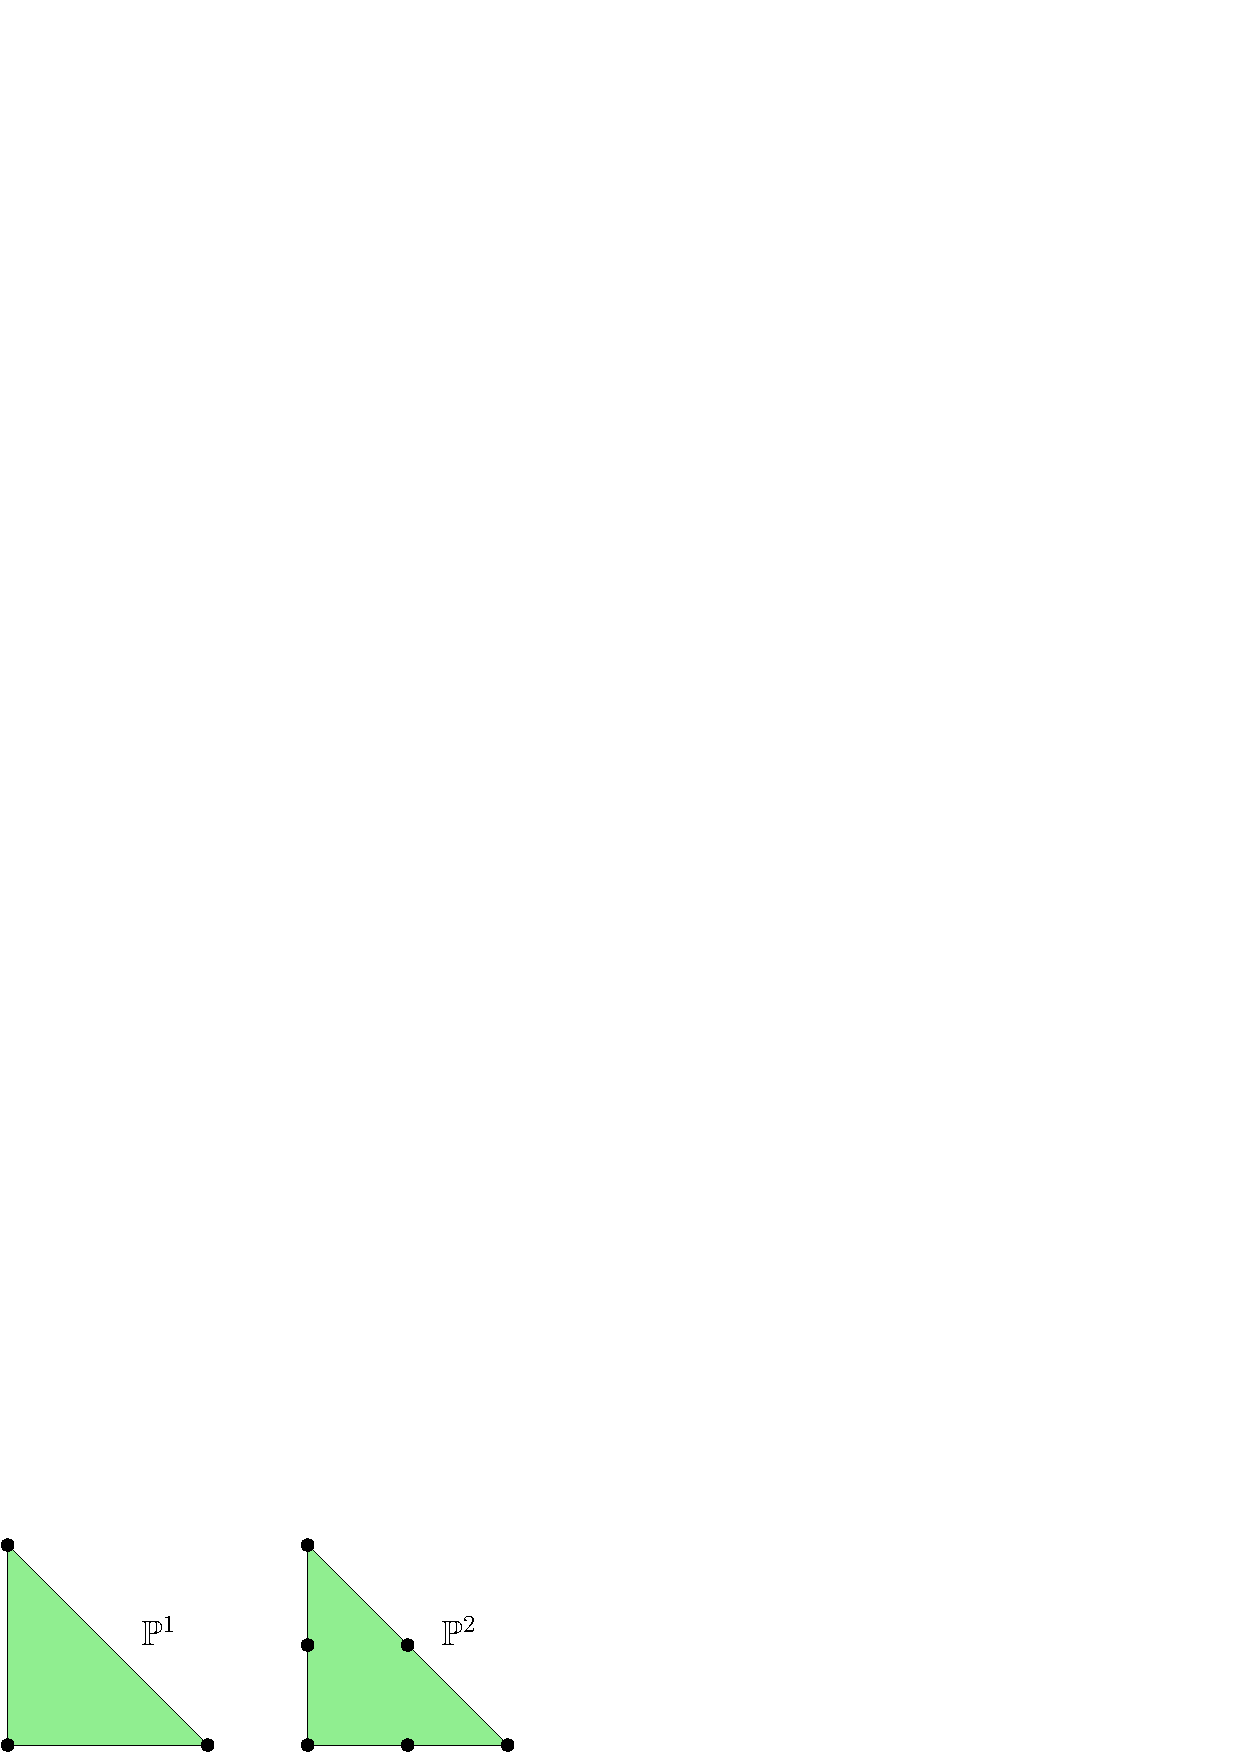
\includegraphics[height=0.2\textheight]{LagrangeP1P2}
\end{block}

\end{frame}

\section{Numerical simulations}


\subsection{Eigenvalues computation}

\begin{frame}{Eigenvalues analysis for a square plate}
Non-dimensional eigenfrequencies:
\begin{equation}
\widehat{\omega}_{mn}^h = \omega_{mn}^h L \left(\frac{2 (1 + \nu) \rho}{E}\right)^{1/2}
\end{equation}
$m$ and $n$ being the numbers of half-waves occurring in the modes shapes in the $x$ and $y$ directions. The only parameters which influence the results are the Poisson's ratio $\nu=0.3$ (fixed) and the thickness-to-span ratio $h/L$. \\
The error is computed by\footfullcite{dawe1980rayleigh}
\begin{equation}
\varepsilon = \frac{\text{abs}(\widehat{\omega}_{mn}^h - \omega_{mn}^{DR})}{\omega_{mn}^{DR}}.
\end{equation}
The eigenproblem is solved using the QR algorithm.

\end{frame}

\begin{frame}{Eigenvalues for the thick case $h/L=0.1$}
\onslide*<1>{
\begin{table}
\footnotesize
\centering	
\begin{tabular}{ccggNb}
	\hline 
	BCs					  & Mode & \cellcolor{white}$N=10$&\cellcolor{white} $N=20$& H-H &\cellcolor{white} D-R \\ 
	\hline 
	\multirow{4}{*}{CCCC} &$\widehat{\omega}_{11}$& 1.5999& 1.5917& 1.591& 1.594\\
	&$\widehat{\omega}_{21}$& 3.0615& 3.0410& 3.039& 3.046\\
	&$\widehat{\omega}_{12}$& 3.0615& 3.0410& 3.039& 3.046\\
	&$\widehat{\omega}_{22}$& 4.3161& 4.2682& 4.263& 4.285\\
	\hline	
	\multirow{4}{*}{SSSS} &$\widehat{\omega}_{11}$& 0.9324& 0.9324& 0.930& 0.930\\
	&$\widehat{\omega}_{21}$& 2.2227& 2.2226& 2.219& 2.219\\
	&$\widehat{\omega}_{12}$& 2.2227& 2.2226& 2.219& 2.219\\
	&$\widehat{\omega}_{22}$& 3.4142& 3.3608& 3.405& 3.406\\
	\hline		
	\multirow{4}{*}{SCSC} &$\widehat{\omega}_{11}$& 1.3111& 1.3013& 1.300& 1.302\\
	&$\widehat{\omega}_{21}$& 2.4155& 2.3966& 2.394& 2.398\\
	&$\widehat{\omega}_{12}$& 2.9082& 2.8871& 2.885& 2.888\\
	&$\widehat{\omega}_{22}$& 3.8906& 3.8458& 3.839& 3.852\\
	\hline
	\multirow{5}{*}{CCCF} &$\widehat{\omega}_{\frac{1}{2}1}$& 1.0855& 1.0982&	1.081&	1.089\\
	&$\widehat{\omega}_{\frac{3}{2}1}$& 1.7636& 1.7461&	1.744&	1.758\\
	&$\widehat{\omega}_{\frac{1}{2}2}$& 2.6696& 2.6575&	2.657&	2.673\\
	&$\widehat{\omega}_{\frac{5}{2}1}$& 3.2248& 3.1997&	3.197&	3.216\\
	\hline 
\end{tabular} 	
\caption{Eigenvalues for $h/L = 0.1$ using $\mathbb{P}_1$: \\
	\sqbox{Blue} reference, \, \sqbox{Green} $\varepsilon<2\%$. }
\label{tab:thin}
\end{table}
}

\onslide*<2>{
	\begin{table}
		\footnotesize
		\centering
		\begin{tabular}{ccggNb}
			\hline 
			BCs	& Mode & \cellcolor{white}$N=5$ & \cellcolor{white}$N=10$& H-H &\cellcolor{white} D-R \\ 
			\hline
			\multirow{4}{*}{CCCC} &$\widehat{\omega}_{11}$& 1.5976&	1.5914&	1.591&	1.594\\ 
			&$\widehat{\omega}_{21}$& 3.0584&	3.0405&	3.039&	3.046\\ 
			&$\widehat{\omega}_{12}$& 3.0677&	3.0405& 3.039&	3.046\\ 
			&$\widehat{\omega}_{22}$& 4.3109&	4.2662&	4.263&	4.285\\ 
			\hline 		
			\multirow{4}{*}{SSSS} &$\widehat{\omega}_{11}$& 0.9304&	0.9302&	0.930&	0.930\\ 
			&$\widehat{\omega}_{21}$& 2.2223&	2.2194&	2.219&	2.219\\ 
			&$\widehat{\omega}_{12}$&	2.2224&	2.2194& 2.219&	2.219\\ 
			&$\widehat{\omega}_{22}$& 3.4128&	3.4061&	3.405&	3.406\\		
			\hline 
			\multirow{4}{*}{SCSC} &$\widehat{\omega}_{11}$& 1.3053&	1.3004&	1.300&	1.302\\
			&$\widehat{\omega}_{21}$& 2.4040&	2.3946&	2.394&	2.398\\
			&$\widehat{\omega}_{12}$& 2.9060& 2.8858&	2.885&	2.888\\
			&$\widehat{\omega}_{22}$& 3.8721&	3.8415&	3.839&	3.852\\
			\hline 		
			\multirow{4}{*}{CCCF} &$\widehat{\omega}_{\frac{1}{2}1}$& 1.0845& 1.0797& 1.081& 1.089\\
			&$\widehat{\omega}_{\frac{3}{2}1}$& 1.7559& 1.7425& 1.744& 1.758\\	
			&$\widehat{\omega}_{\frac{1}{2}2}$& 2.6762& 2.6547& 2.657& 2.673\\
			&$\widehat{\omega}_{\frac{5}{2}1}$& 3.2186& 3.1954& 3.197& 3.216\\		
			\hline 
		\end{tabular} 
		\captionsetup{width=0.95\linewidth}
		\captionof{table}{Eigenvalues for $h/L = 0.1$ using $\mathbb{P}_2$: \\
			\sqbox{Blue} reference, \, \sqbox{Green} $\varepsilon<2\%$,\, \sqbox{GreenYellow} $\varepsilon<5\%$, \, 	
			\sqbox{Yellow} $\varepsilon<15\%$.}
	\end{table}
}
\end{frame}

\begin{frame}{Eigenvalues for the thin case $h/L=0.01$}
\onslide*<1>{
	\begin{table}
		\footnotesize
		\centering	
		\begin{tabular}{ccccNb}
			\hline 
			BCs					  & Mode &\cellcolor{white}$N=10$&\cellcolor{white}$N=20$& H-H &\cellcolor{white} D-R \\ 
			\hline 
			\multirow{4}{*}{CCCC} &$\widehat{\omega}_{11}$& \cellcolor{Yellow}0.1967&\cellcolor{Green}0.1765&	0.1754&	0.1754\\
			&$\widehat{\omega}_{21}$& \cellcolor{Yellow}0.4030&	\cellcolor{Green}0.3604&	0.3574&	0.3576\\
			&$\widehat{\omega}_{12}$& \cellcolor{Yellow}0.4030&	\cellcolor{Green}0.3604&	0.3574&	0.3576\\
			&$\widehat{\omega}_{22}$& \cellcolor{Orange}0.6431&	\cellcolor{Green}0.5358&	0.5264&	0.5274\\
			\hline 	
			\multirow{4}{*}{SSSS} &$\widehat{\omega}_{11}$&	\cellcolor{Red}0.1706&\cellcolor{Orange}0.1128&	0.0963&	0.0963\\
			&$\widehat{\omega}_{21}$&	\cellcolor{Purple}0.3576&\cellcolor{Yellow}0.2660&	0.2406&	0.2406\\
			&$\widehat{\omega}_{12}$&	\cellcolor{Purple}0.3576&\cellcolor{Yellow}0.2660&	0.2406&	0.2406\\
			&$\widehat{\omega}_{22}$&	\cellcolor{Purple}0.5803&\cellcolor{Orange}0.4442&	0.3847&	0.3848\\
			\hline 			
			\multirow{4}{*}{SCSC} &$\widehat{\omega}_{11}$&	\cellcolor{Purple}0.1864&\cellcolor{Yellow}0.1487&	0.1411&	0.1411\\
			&$\widehat{\omega}_{21}$&	\cellcolor{Purple}0.3649&\cellcolor{Yellow}0.2829&	0.2668&	0.2668\\
			&$\widehat{\omega}_{12}$&	\cellcolor{Orange}0.3987&\cellcolor{GreenYellow}0.3485&	0.3377&	0.3377\\
			&$\widehat{\omega}_{22}$&	\cellcolor{Purple}0.6075&\cellcolor{Yellow}0.4933&	0.4604&	0.4608\\
			\hline 		
			\multirow{5}{*}{CCCF} &$\widehat{\omega}_{\frac{1}{2}1}$& \cellcolor{Yellow}0.1238& \cellcolor{Green}0.1166&0.1166&0.1171\\
			&$\widehat{\omega}_{\frac{3}{2}1}$& \cellcolor{Yellow}0.2207& \cellcolor{Green}0.1954&	0.1949&	0.1951\\
			&$\widehat{\omega}_{\frac{1}{2}2}$& \cellcolor{GreenYellow}0.3204& \cellcolor{Green}0.3078&	0.3080&	0.3093\\
			&$\widehat{\omega}_{\frac{5}{2}1}$& \cellcolor{Yellow}0.4144& \cellcolor{Green}0.3751&	0.3736&	0.3740\\			
			\hline 
		\end{tabular} 
		\captionsetup{width=0.95\linewidth}
		\captionof{table}{Eigenvalues for $h/L = 0.01$ using $\mathbb{P}_1$:	
			\sqbox{Blue} reference, \, \sqbox{Green} $\varepsilon<2\%$, \, \\ \sqbox{GreenYellow} $\varepsilon<5\%$, \, 	
			\sqbox{Yellow} $\varepsilon<15\%$, \, \sqbox{Orange} $\varepsilon<30\%$, \, \sqbox{Purple} $\varepsilon<50\%$,	
			\, \sqbox{Red} $\varepsilon<80\%$.
		}
\end{table}
}

\onslide*<2>{
\begin{table}[h]
	\footnotesize
	\centering
	\begin{tabular}{ccmgNb}
		\hline 
		BCs					  & Mode & \cellcolor{white}$N=5$ & \cellcolor{white}$N=10$ & H-H & \cellcolor{white} D-R \\ 
		\hline
		\multirow{4}{*}{CCCC} &$\widehat{\omega}_{11}$& 0.1872&	0.1762&	0.1754&	0.1754\\ 
		&$\widehat{\omega}_{21}$& \cellcolor{GreenYellow}0.3725&	0.3598&	0.3574&	0.3576\\ 
		&$\widehat{\omega}_{12}$& 0.4055&0.3598&0.3574&	0.3576\\ 
		&$\widehat{\omega}_{22}$& 0.6043&0.5335&0.5264&	0.5274\\ 	
		\hline 		
		\multirow{4}{*}{SSSS} &$\widehat{\omega}_{11}$& \cellcolor{Green}0.0963&	0.0963&	0.0963&	0.0963\\ 
		&$\widehat{\omega}_{21}$& \cellcolor{Green}0.2422&	0.2406&	0.2406&	0.2406\\ 
		&$\widehat{\omega}_{12}$& \cellcolor{Green}0.2430&	0.2406&	0.2406&	0.2406\\ 
		&$\widehat{\omega}_{22}$& \cellcolor{Green}0.3874&	0.3848&	0.3847&	0.3848\\ 		
		\hline 
		\multirow{4}{*}{SCSC} &$\widehat{\omega}_{11}$& 0.1492&	0.1418&	0.1411&	0.1411\\ 
		&$\widehat{\omega}_{21}$& 0.2827&	0.2683&	0.2668&	0.2668\\ 
		&$\widehat{\omega}_{12}$& 0.3608&	0.3394&	0.3377&	0.3377\\ 
		&$\widehat{\omega}_{22}$& 0.4940&	0.4654&	0.4604&	0.4608\\ 
		\hline 		
		\multirow{4}{*}{CCCF} &$\widehat{\omega}_{\frac{1}{2}1}$& \cellcolor{GreenYellow}0.1197& 0.1169& 0.1166& 0.1171\\ 
		&$\widehat{\omega}_{\frac{3}{2}1}$& 0.2092& 0.1960& 0.1949& 0.1951\\ 	
		&$\widehat{\omega}_{\frac{1}{2}2}$& \cellcolor{GreenYellow}0.3188& 0.3089& 0.3080& 0.3093\\ 
		&$\widehat{\omega}_{\frac{5}{2}1}$& 0.3938& 0.3757& 0.3736& 0.3740\\ 
		\hline 
	\end{tabular} 
	\captionsetup{width=0.95\linewidth}
	\captionof{table}{Eigenvalues for $h/L = 0.01$ using $\mathbb{P}_2$: \\
		\sqbox{Blue} reference, \, \sqbox{Green} $\varepsilon<2\%$,\, \sqbox{GreenYellow} $\varepsilon<5\%$, \, 	
		\sqbox{Yellow} $\varepsilon<15\%$.}
\end{table}
}
\end{frame}


\subsection{Time domain simulations}

\begin{frame}{Settings for time domain simulation}

We consider a square plate under different BCs and external excitations.

\begin{itemize}
\item Finite element space $\mathbb{P}_2$;
\item Number of finite elements $10 \times 10$;
\item Integrator St\"ormer-Verlet;
\item Integration step $1 [\mu s]$;
\item Total simulation time $t_{\text{fin}} = 10 [ms]$. 
\end{itemize}

\end{frame}

\begin{frame}{First simulation}
\onslide*<1>{
Boundary conditions:
\begin{itemize}
	\item $x=0 \rightarrow$ Clamped,
	\item $x=1 \rightarrow$ Free,
	\item $y=0 \rightarrow q_n = f(t), \, m_{nn} = m_{ns}= 0$,
	\item $y=1 \rightarrow q_n = -f(t), \, m_{nn} = m_{ns}= 0$,
\end{itemize}
where 
\begin{equation}
f(t) = \begin{cases}
10^6 \; [Pa \cdot m], \; &\forall t< 0.25 \, t_{\text{fin}}, \\
0, \; &\forall t\geq 0.25 \, t_{\text{fin}}. \\
\end{cases}
\end{equation}
}
\begin{center}
\onslide*<2>{
\movie[width=0.9\textwidth, height = 0.7 \textheight]{Simulation 1}{./Videos/Video_n1.mp4}	
}


\onslide*<3>{
\includegraphics[width=0.8\textwidth]{Sim1Hamiltonian.eps}
}
\end{center}
\end{frame}


\begin{frame}{Second simulation}
\onslide*<1>{
Boundary conditions:
The set of BC for the second simulation is
\begin{itemize}
	\item $x=0 \rightarrow$ Clamped,
	\item $x=1 \rightarrow q_n = g(y, t), \, m_{nn} = m_{ns}= 0$,
	\item $y=0 \rightarrow$ Clamped,
	\item $y=1 \rightarrow$ Clamped,
\end{itemize}
where 
\begin{equation}
g(y, t) = \begin{cases}
10^6 \, \sin \left( \frac{2 \pi}{L} y \right) \; [Pa \cdot m], \; &\forall t< 0.1 \, t_{\text{fin}}, \\
0, \; &\forall t\geq 0.1 \, t_{\text{fin}}. \\
\end{cases}
\end{equation}
}
\begin{center}
\onslide*<2>{
	\movie[width=0.9\textwidth, height = 0.7 \textheight]{Simulation 2}{./Videos/Video_n2.mp4}	
}
	\onslide*<3>{
		\includegraphics[width=0.8\textwidth]{Sim2Hamiltonian.eps}
	}
\end{center}
\end{frame}

\begin{frame}{Third simulation}
\onslide*<1>{
Clamped plate subjected to gravity	
}
\begin{center}
\onslide*<1>{
			\movie[width=0.9\textwidth, height = 0.7 \textheight]{Simulation 3}{./Videos/Video_n3.mp4}	
	}
	\onslide*<2>{
		\includegraphics[width=0.8\textwidth]{Sim3Hamiltonian.eps}
	}
\end{center}
\end{frame}

\section{Conclusion}
\begin{frame}{Conclusion}
Present and future developments:
\begin{itemize}
\item extend the port Hamiltonian formalism to thin plate\footfullcite{BrugnoliKir};
\item model reduction for pHDAE of second order\footfullcite{Mehrmann2018};
\end{itemize}
\end{frame}

\begin{frame}
\centering
Thank you for your attention. Questions?
\end{frame}


\begin{frame}[allowframebreaks]{References}
\printbibliography
\end{frame}




\end{document}
